\documentclass[]{beamer}
\mode<presentation>{
  %% \usetheme[compress]{Berlin}
}
%% packages
\usepackage{zhspacing}
\zhspacing
\usepackage{graphics}
\usepackage{listings}
\lstset{basicstyle=\ttfamily\footnotesize}
\usepackage{tabularx}
\usepackage{booktabs}
%% meta info
\title{Clang ASTMatcher: Workflow in Detail}
%\subtitle{An Introduction}
\author[SuXing~pysuxing@gmail.com]{SuXing}
\institute{TOW}
\date{\today}

%% slides
\begin{document}
\setlength{\parindent}{0pt}

\frame{\titlepage}

\frame{\tableofcontents}

\section{AST Type Hierarchy}
\frame{\tableofcontents[currentsection]}

\begin{frame}
  \frametitle{Type Hierarchy}
  The Clang AST contains hundreds of node types, forming a
  multi-root(9 roots) type hierarchy
  \pause
  \begin{columns}
    \begin{column}{.5\textwidth}
      \begin{itemize}
        \item CXXCtorInitializer
        \item TemplateArgument
        \item NestedNameSpecifier
        \item NestedNameSpecifierLoc
        \item QualType
      \end{itemize}
    \end{column}
    \begin{column}{.5\textwidth}
      \begin{itemize}
        \item TypeLoc
        \item \alert{Decl}
        \item \alert{Stmt}
        \item \alert{Type}
      \end{itemize}
    \end{column}
  \end{columns}
  \pause
  Each AST node type has an integer ID, from which type inheritances can
  be determind at runtime
\end{frame}

\begin{frame}
  \frametitle{Dynamic-typed Node}
  class \alert{DynTypedNode}, as described in its doc
  \begin{quotation}
    A dynamically typed AST node container.
    Stores an AST node in a type safe way.
    This allows writing code that works with different
    kinds of AST nodes, despite the fact that they don't
    have a common base class.
  \end{quotation}
  \pause
  \lstinputlisting[language=C++]{listings/dyntypednode.cpp}
\end{frame}

\begin{frame}
  \frametitle{Dynamic-typed Node (cont.)}
  AST nodes are stored in \alert{DynTypedNode} object by
  \begin{itemize}
    \item dynamic cast pointer\\
      Decl, Stmt, Type and their subclasses
    \item pointer\\
      NestedNameSpecifier, CXXCtorInitializer, TemplateArgument
    \item value\\
      NestedNameSpecifierLoc, QualType, TypeLoc
  \end{itemize}
\end{frame}

\section{Workflow of AST Node Matching}
\frame{\tableofcontents[currentsection]}

\begin{frame}
  \frametitle{How matchers work?}
  Use the \texttt{MatchFinder} class.
  \begin{itemize}
    \item \texttt{void addMatcher(Matcher<...>\&, MatchCallBack*)}\\
      %% Register a matcher object with a callback object,
      %% overloaded for all six AST node types (recall)
    \item \texttt{MatchFinder::MatchResult}\\
      %% Containing infomation of matched AST nodes.
    \item \texttt{MatchFinder::MatchCallBack}\\
      \texttt{void MatchCallBack::run(MatchResult\&)}\\
      %% Inner class with a \texttt{run} method. Every time a match is found,
      %% The \texttt{MatchFinder} will invoke the registered \texttt{MatchCallBack} object,
      %% passing it a \texttt{MatchResult} object
  \end{itemize}
\end{frame}

\begin{frame}
  \frametitle{Typical design of Clang tools}
  \begin{figure}
    \includegraphics[width=.8\textwidth]{figures/clangtool-structure}
  \end{figure}
\end{frame}

\begin{frame}
  \frametitle{Inject matchers into Clang Tool structure}
  The \texttt{MatchFinder} class defines the \alert{newASTConsumer} method,
  so we can create a \texttt{FrontendActionFactory} object with a \texttt{MatchFinder} object.
  \lstinputlisting[language=C++]{listings/matchfinder.cpp}
  \texttt{MatchFinder} is yet another kind of \texttt{FrontendAction}!
\end{frame}

\begin{frame}
  \frametitle{Recall: Typical design of Clang tools}
  \begin{figure}
    \includegraphics[width=.8\textwidth]{figures/clangtool-structure}
  \end{figure}
\end{frame}

\begin{frame}
  \frametitle{Call Graph of Node Matching}
  \begin{figure}
    \includegraphics[height=.7\textheight]{figures/callgraph}
  \end{figure}
\end{frame}

\begin{frame}
  \frametitle{AST matche example: step by step}
  \lstinputlisting[language=C++]{listings/example-comment.cpp}
\end{frame}

%% \section{AST Matchers and Matcher Creators}
%% \frame{\tableofcontents[currentsection]}

%% \begin{frame}
%%   \frametitle{Review: AST matcher categories}
%%   AST matchers are categorized as
%%   \begin{itemize}
%%     \item Node Matchers\\
%%       Matchers that match a specific type of AST node
%%     \item Narrowing Matchers\\
%%       Matchers that match attributes on AST nodes
%%     \item Traversal Matchers\\
%%       Matchers that allow traversal between AST nodes
%%   \end{itemize}
%% \end{frame}

%% \begin{frame}
%%   \frametitle{Node Matchers}
%%   All Node matcher creators take several($\geq{}1$) Matchers and return
%%   one Matcher
%%   \begin{figure}
%%     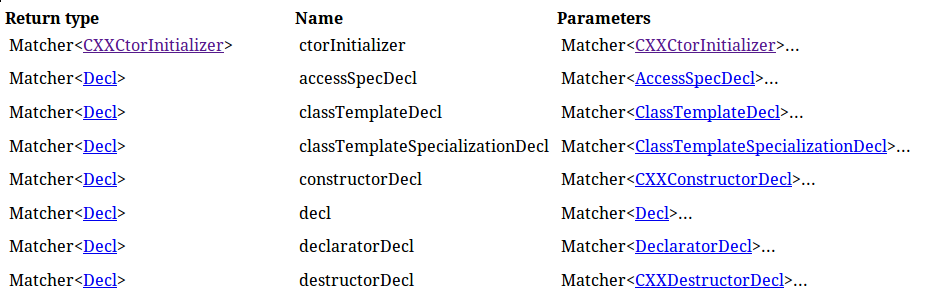
\includegraphics[width=\textwidth]{figures/matchers-prototype}
%%   \end{figure}
%% \end{frame}

%% \begin{frame}
%%   \frametitle{Traversal and Narrowing Matchers}
%%   All Node matcher creators take several($\geq{}1$) Matchers and return
%%   one Matcher
%%   \begin{figure}
%%     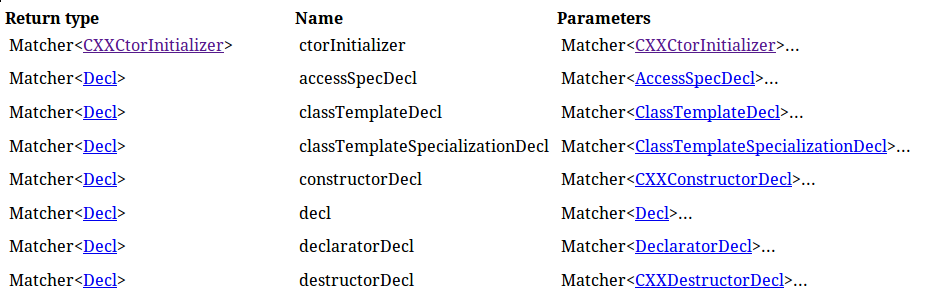
\includegraphics[width=\textwidth]{figures/matchers-prototype}
%%   \end{figure}
%% \end{frame}

\section{Summary}
\frame{\tableofcontents[currentsection]}

\begin{frame}
  \frametitle{Summary}
  \begin{itemize}
    \item AST Type Hierarchy\\
      9-root type hierarchy
    \item Workflow of AST Node Matching\\
      structure of clang tools and how Matchers are injected in\\
      internal mechanism of Matchers (the outside-to-inside order)
  \end{itemize}
\end{frame}

\begin{frame}
  \frametitle{References}
  \begin{itemize}
    \item http://clang.llvm.org/docs/LibASTMatchersReference.html
    \item Source code
      \begin{itemize}
        \item \alert{include/clang/ASTMatchers/ASTMatchersInternal.h}
        \item include/clang/ASTMatchers/ASTMatchersMacros.h
        \item include/clang/ASTMatchers/ASTMatchers.h
        \item include/clang/ASTMatchers/ASTMatchFinder.h
        \item \alert{lib/ASTMatchers/ASTMatchFinder.cpp}
      \end{itemize}
  \end{itemize}
\end{frame}

\frame{\centerline{\Huge Q\&A}}

\end{document}
